\subsubsection{Taxi density distribution}
\label{section_taxi_denstiy_distribution}

To validate $assumption 2$, we quantitatively analyze vehicles density in one hour. By dividing the whole network into $100*100$ grids, taxi density distributions for event 0, 1 and 4 are computed in each cell. As shown in table \ref{table_event_detail}, event 4 means no event, that is, a taxi uploads its GPS information every 60 minutes and set the event as 4. As fig.\ref{figure_taxi_density_for_one_hour}.(d), (e), (f), it is obvious that the taxi density for event 4 is higher than for other events reaching up to $600 vehicles/cell$. The taxi density of cells on roads stayed in a relatively high level. Nevertheless, for event 1, the taxi density of most cells is less than 5, which means that less than 5 taxis during the time period took passengers in those locations, while the high dense cells occurred sparsely. By further exploring some high dense cells, it can be found that hot cells for event 0 and 1 include Beijing Train station, the junction of the south 4th Ring Road and subway line one in Beijing, China.


\begin{figure*}[htbp]
\centering
\subfigure[$event=1,7:00-8:00$]{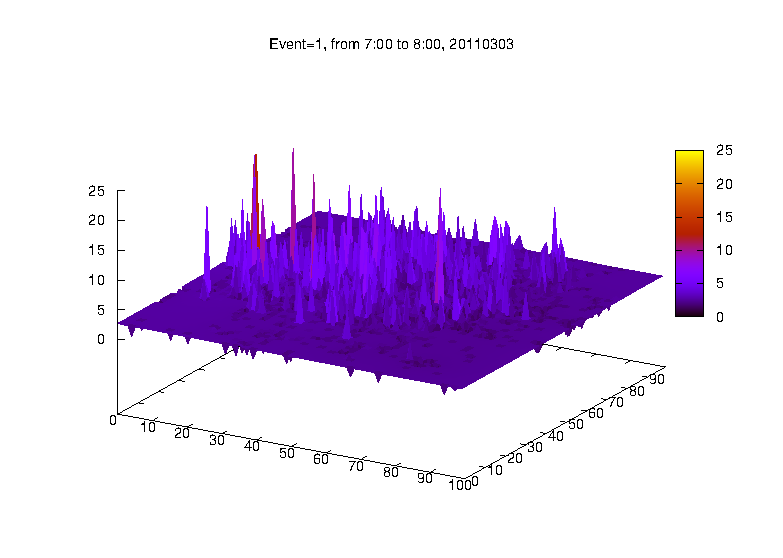
\includegraphics[width=0.3\textwidth]{figures_201103/Event=1_7_8_20110303.eps}}
\subfigure[$event=1,12:00-13:00$]{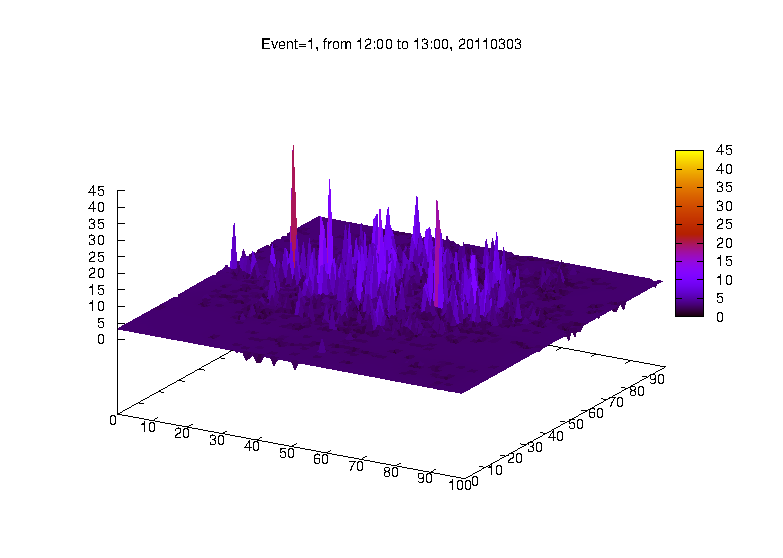
\includegraphics[width=0.3\textwidth]{figures_201103/Event=1_12_13_20110303.eps}}
\subfigure[$event=1,17:00-18:00$]{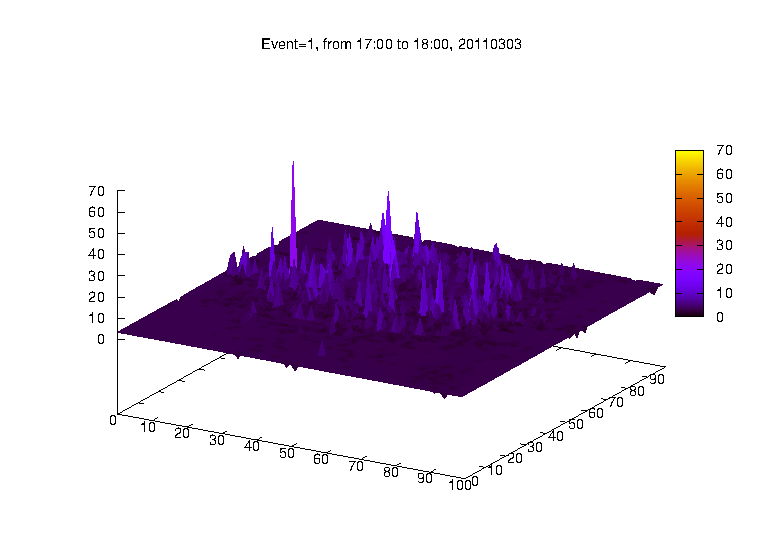
\includegraphics[width=0.3\textwidth]{figures_201103/Event=1_17_18_20110303.eps}}
\subfigure[$event=4,7:00-8:00$]{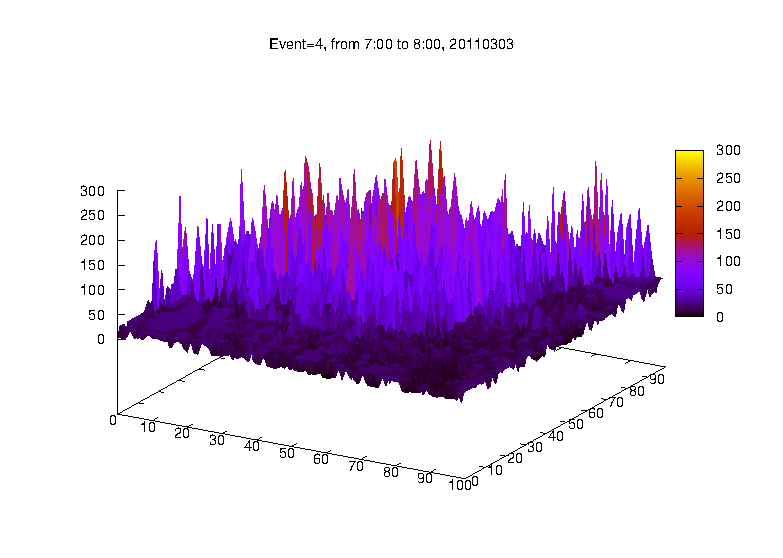
\includegraphics[width=0.3\textwidth]{figures_201103/Event=4_7_8_20110303.eps}}
\subfigure[$event=4,12:00-13:00$]{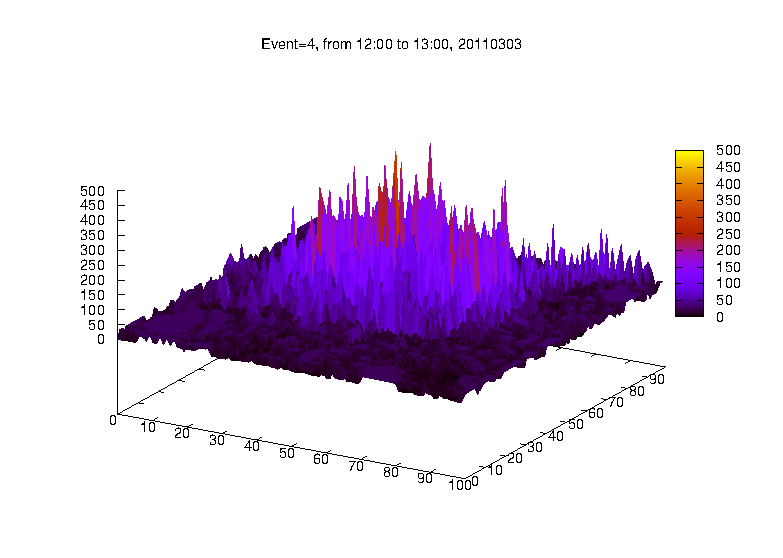
\includegraphics[width=0.3\textwidth]{figures_201103/Event=4_12_13_20110303.eps}}
\subfigure[$event=4,17:00-18:00$]{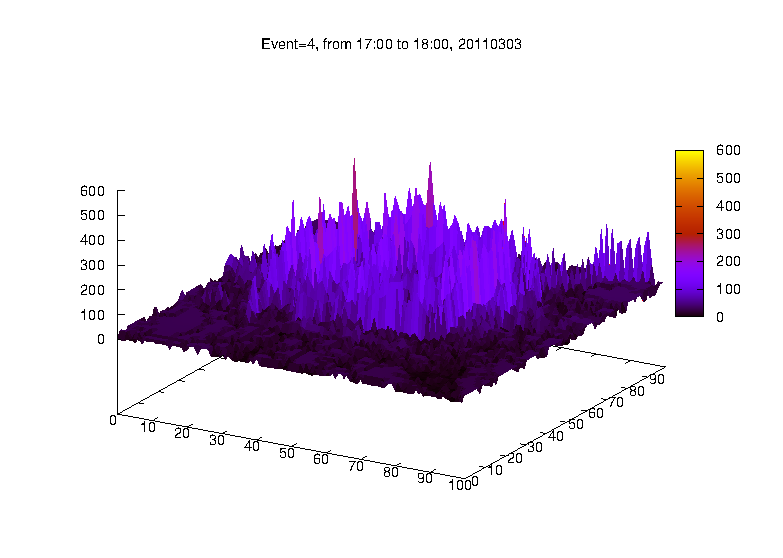
\includegraphics[width=0.3\textwidth]{figures_201103/Event=4_17_18_20110303.eps}}

\caption{Taxi density for event 1 and 4 in one hour}\label{figure_taxi_density_for_one_hour}
\end{figure*}

The taxi density distributions for event 1 from March 3th to March 7th are plot in fig.\ref{figure_taxi_density_for_5days}. The crest value is about 50. And the position of peaks are similar. Fig.\ref{figure_taxi_density_for_5days}.(c) demonstrates some difference. It may be caused by that it is Sunday and many people should return to the city and prepare for work next day.

\begin{figure*}[htbp]
\centering

\subfigure[$event=1,12:00-13:00,2011/03/03$]{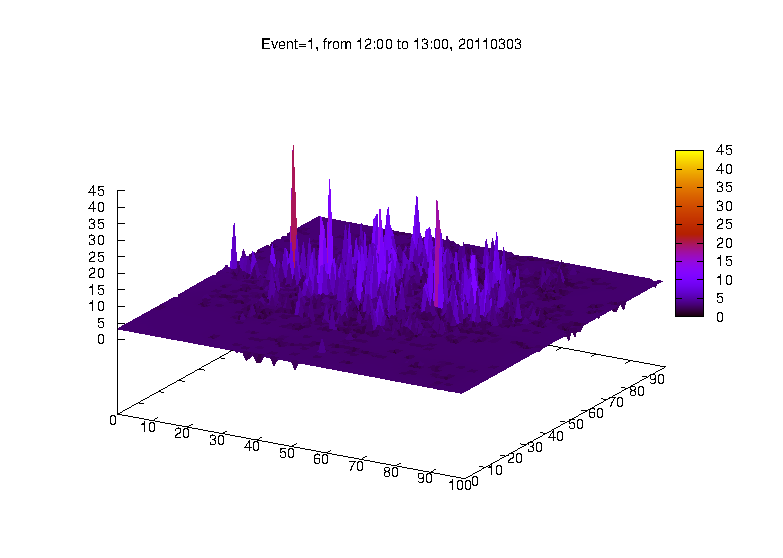
\includegraphics[width=0.3\textwidth]{figures_201103/Event=1_12_13_20110303.eps}}
\subfigure[$event=1,12:00-13:00,2011/03/04$]{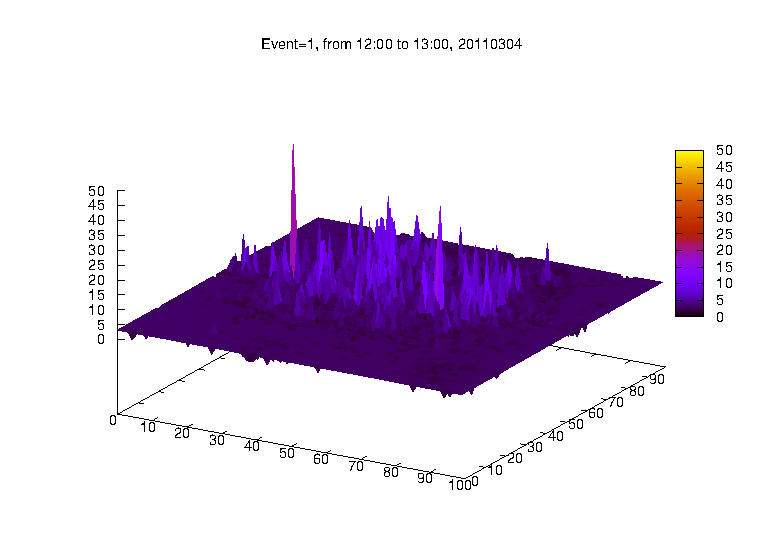
\includegraphics[width=0.3\textwidth]{figures_201103/20110304120000.eps}}
\subfigure[$event=1,12:00-13:00,2011/03/05$]{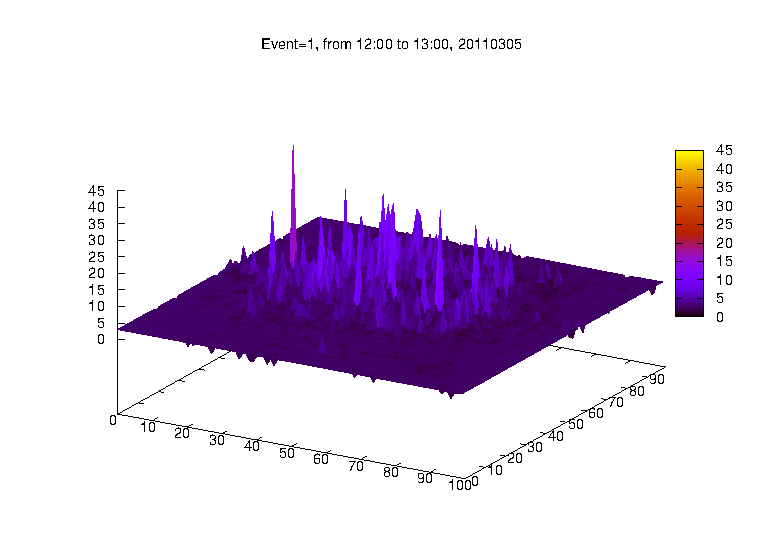
\includegraphics[width=0.3\textwidth]{figures_201103/20110305120000.eps}}
\subfigure[$event=1,12:00-13:00,2011/03/06$]{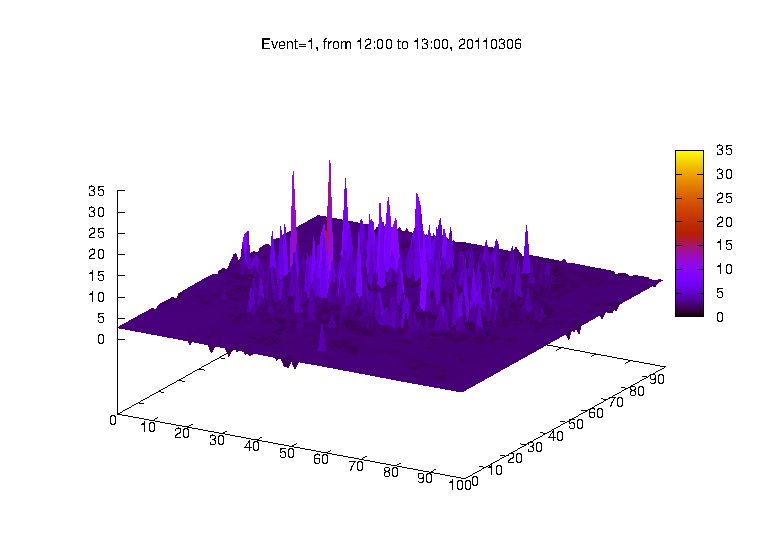
\includegraphics[width=0.3\textwidth]{figures_201103/20110306120000.eps}}
\subfigure[$event=1,12:00-13:00,2011/03/07$]{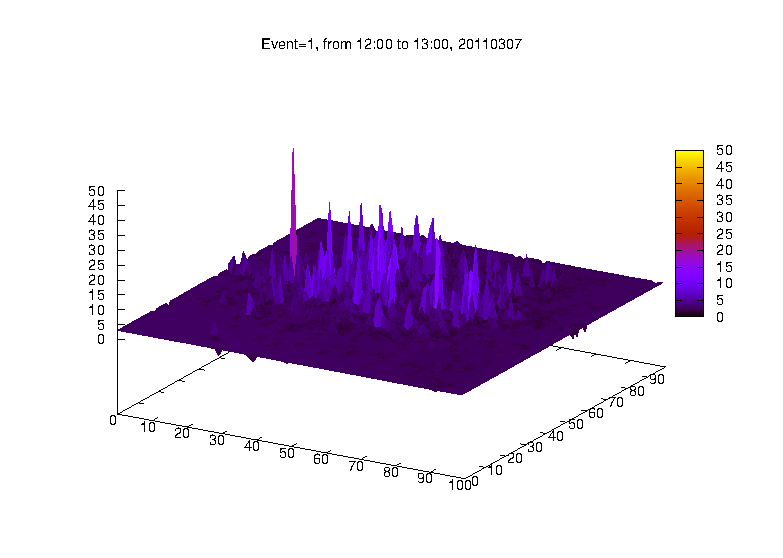
\includegraphics[width=0.3\textwidth]{figures_201103/20110307120000.eps}}
\caption{Taxi density for event 1 in one hour from 03/03 to 03/07, 2011}\label{figure_taxi_density_for_5days}
\end{figure*}

The amount of loading passengers in each cell shows geographic feathers and the distribution is uneven, which support the \emph{assumption 2}. 